
\documentclass[conference]{IEEEtran}

\usepackage[utf8]{inputenc}
\usepackage[T1]{fontenc}
\usepackage{amsmath}
\usepackage{amssymb}
\usepackage{graphicx}
\usepackage{booktabs}
\usepackage{array}
\usepackage{url}
\usepackage{multirow}
\usepackage{float}
\usepackage{placeins}

\newcommand{\code}[1]{\texttt{#1}}

\title{Semantic Label-to-Image Synthesis for TU-Graz Landing with Conditional GANs}

\author{
\IEEEauthorblockN{Erik Figueiral Alonso, Roi Cores Cabaleiro}
\IEEEauthorblockA{Computer Vision II\\
Submission package: \code{CV2\_ASSIGMENT\_GAN}}
}

\begin{document}
\maketitle

\begin{abstract}
This project studies conditional image generation for the TU-Graz Landing dataset. The input is a semantic label map and the desired output is a plausible aerial RGB image. We implement a clean PyTorch framework around Pix2Pix, LSGAN, self-attention Pix2Pix, Pix2PixHD-lite, and a transfer-learning ResNet-U-Net variant. The code uses shared dataset, model, training, inference, and metric abstractions so that variants differ only where the experiment requires it. Completed runs show that Pix2PixHD-lite obtains the best validation MAE among the finished models, while LSGAN obtains the strongest SSIM. A time-limited 50-epoch ablation batch tests lower reconstruction weight, L2 reconstruction, attention, and reduced Pix2PixHD feature matching. The report emphasizes both quantitative metrics and qualitative inspection, because the semantic input removes texture and lighting information and makes exact RGB reconstruction ambiguous.
\end{abstract}

\section{Introduction}
Generative adversarial networks (GANs) learn a generator and a discriminator in a two-player game~\cite{goodfellow2014gan}. The generator maps a latent or conditional input to a synthetic sample, while the discriminator estimates whether a sample comes from the real data distribution. In the original GAN formulation, the optimal discriminator has the form
\begin{equation}
D^*(x)=\frac{p_{data}(x)}{p_{data}(x)+p_g(x)},
\end{equation}
which makes the training objective a distribution-matching problem rather than a simple pixel-regression problem. This idea is useful for image synthesis because realism is not fully captured by a per-pixel loss.

The assigned task is not semantic segmentation. A segmentation model would map an RGB image to a label map. Here the direction is reversed: the model receives a semantic label map and synthesizes an RGB aerial image. This conditional image-to-image setting is naturally modeled with Pix2Pix~\cite{isola2017pix2pix}. A U-Net generator preserves the spatial layout of the condition through skip connections, and a PatchGAN discriminator judges whether local patches of the generated image look compatible with the label map.

This problem is ambiguous. A label map tells the model where grass, pavement, people, or obstacles are, but it does not specify exact texture, shadows, lighting, color variation, or fine object appearance. Therefore, a deterministic U-Net can be competitive in paired metrics, especially MAE, but it tends to predict averaged textures. The adversarial component is included because the project objective is generative synthesis: the output should not only be close to one paired target, but also look locally plausible.

\section{Related Work}
The original GAN paper introduced the adversarial training framework and motivated distribution matching through a discriminator~\cite{goodfellow2014gan}. DCGAN later established practical convolutional design rules for visual GANs: strided convolutions instead of pooling, normalization for stable optimization, ReLU-like activations in the generator, LeakyReLU in the discriminator, and a bounded generator output such as \code{tanh}~\cite{radford2016dcgan}. Conditional GANs extend GANs by conditioning both generator and discriminator on external information such as class labels or images~\cite{mirza2014cgan}. Pix2Pix applies this idea to paired image-to-image translation~\cite{isola2017pix2pix}.

Several variants address GAN instability and image realism. LSGAN replaces binary cross entropy with least-squares regression targets, often producing smoother gradients~\cite{mao2017lsgan}. Pix2PixHD improves high-resolution conditional synthesis with residual generators, multi-scale discriminators, and feature matching~\cite{wang2018pix2pixhd}. Self-attention adds non-local context, helping convolutional networks reason about distant regions without abandoning convolutional inductive bias~\cite{zhang2019sagan}. Transfer learning can reuse a pretrained visual encoder, for example a ResNet backbone~\cite{he2016resnet}, although this must be adapted carefully because ImageNet pretraining is not directly optimized for label-map-to-aerial-image synthesis.

GAN evaluation is also non-trivial. The course-provided GAN variants material emphasizes that no single universal metric exists for all GAN applications~\cite{ganvariants}. We therefore combine paired metrics, structural similarity, classifier two-sample testing, generative precision/recall, and FID where appropriate.


\section{Design Decisions}
We considered several GAN families before fixing the experimental plan. CycleGAN and DualGAN were not chosen as main models because the dataset is paired: every semantic map is already aligned with its target aerial image. Cycle consistency is most useful when paired examples are unavailable. In our case, using CycleGAN would discard useful supervision and train a harder two-domain problem than necessary.

We also considered training one generator per semantic condition and then combining their outputs. This idea is attractive because each generator could specialize in one class, but it has a serious limitation: isolated class generators do not see the spatial context around borders. For landing images, boundaries are exactly where realism is hardest; pavement-to-grass transitions, small obstacles, and people must be coherent with the surrounding area. A single conditional generator is therefore more appropriate because it receives the full label map and can use neighboring regions to synthesize consistent texture.

The attention experiment was included as a light transformer-inspired direction. A pure transformer would be expensive for the available dataset and GPU budget, but self-attention inside a convolutional generator gives a useful compromise: convolutions keep local spatial bias and attention allows distant regions to interact. This is important because CNN receptive fields grow with depth, but long-range relationships can still be weak, especially near semantic boundaries.

Finally, Pix2PixHD-lite was selected as the strongest architecture-oriented variant because it keeps the paired Pix2Pix formulation while improving the generator and discriminator family. Its residual generator and multi-scale PatchGANs are better aligned with realistic aerial synthesis than simply increasing baseline depth.

\section{Technical Approach}
\subsection{Dataset}
The TU-Graz Landing data used here contains approximately 400 paired samples. Each raw image is a horizontal pair: the left half is the real aerial RGB target and the right half is the semantic label map. The project uses a 70/15/15 split, giving approximately 280 training, 60 validation, and 60 test images. The same split seed is used across all experiments.

The generator receives the semantic map $x$ and predicts an RGB image $G(x)$. During training the real target $y$ is available, so paired losses can be used. At inference time the reference image is optional and is displayed only for comparison in the demo.

\subsection{Clean Software Structure}
The code is organized around reusable Python modules rather than notebook-only logic. The notebook calls the same modules as the command-line runners, which makes the delivery reproducible.

\begin{figure}[H]
\centering
\resizebox{\columnwidth}{!}{%
\begin{tabular}{p{0.30\textwidth}p{0.34\textwidth}p{0.34\textwidth}}
\toprule
Experiment hierarchy & Training and model layer & Evaluation and demo layer \\
\midrule
\code{BasePix2PixExperiment} & \code{PairedImageDatasetConfig} & \code{EvaluationContext} \\
$\rightarrow$ \code{BaselinePix2PixExperiment} & $\rightarrow$ \code{PairedTranslationDataset} & $\rightarrow$ \code{PixelStructureMetricsHandler} \\
$\rightarrow$ \code{LSGANExperiment} & $\rightarrow$ \code{UNetGenerator} & $\rightarrow$ \code{DistributionMetricsHandler} \\
$\rightarrow$ \code{AttentionPix2PixExperiment} & $\rightarrow$ \code{AttentionUNetGenerator} & $\rightarrow$ \code{PerceptualMetricsHandler} \\
$\rightarrow$ \code{Pix2PixHDLiteExperiment} & $\rightarrow$ \code{GlobalResnetGenerator} & \code{run\_metric\_chain} \\
$\rightarrow$ \code{TransferLearningExperiment} & $\rightarrow$ \code{ResNetUNetGenerator} & \code{demo.infer.load\_generator} \\
 & $\rightarrow$ \code{PatchGANDiscriminator} & \code{demo.visual\_demo.CheckpointOption} \\
 & $\rightarrow$ \code{MultiscalePatchGANDiscriminator} & \\
 & $\rightarrow$ \code{Pix2PixLosses} & \\
\bottomrule
\end{tabular}}
\caption{Class architecture used by the delivery code. Concrete experiments inherit shared defaults from \code{BasePix2PixExperiment}; model variants are isolated in their own generator classes; metrics are composed as a Chain of Responsibility.}
\label{fig:class-architecture}
\end{figure}
\FloatBarrier

\begin{table}[H]
\caption{Main delivery modules.}
\label{tab:modules}
\centering
\scriptsize
\begin{tabular}{p{0.36\columnwidth}p{0.56\columnwidth}}
\toprule
Module & Role \\
\midrule
\code{dataset.py} & Paired reader, splits, transforms. \\
\code{models.py} & U-Net generator and PatchGAN. \\
\code{models\_attention.py} & U-Net with self-attention bottleneck. \\
\code{models\_pix2pixhd.py} & Residual generator and multi-scale PatchGAN. \\
\code{models\_transfer.py} & ResNet18 encoder adapter. \\
\code{losses.py} & Vanilla GAN, LSGAN, L1 and L2 losses. \\
\code{metric\_chain.py} & Chain of Responsibility for metrics. \\
\code{run\_experiment.py} & Named experiment entry point. \\
\code{visual\_demo.py} & Gradio demo with checkpoint discovery. \\
\bottomrule
\end{tabular}
\end{table}
\FloatBarrier


\subsection{Model Variants}
The first model is the baseline Pix2Pix system. It uses a U-Net generator and a PatchGAN discriminator. The U-Net is appropriate because the input and output are spatially aligned: the road, grass, people, and obstacles should remain in the same positions. Skip connections allow the decoder to recover local structure from early encoder features instead of reconstructing the whole image only from the bottleneck. The PatchGAN discriminator does not classify the whole image with one score; it judges local patches, which is useful for texture realism and semantic boundaries.

The LSGAN variant keeps the same generator and discriminator but changes the adversarial objective. Instead of binary cross entropy, the discriminator is trained with least-squares targets. We included it because the original GAN loss can saturate and produce unstable gradients. In practice, LSGAN often makes training smoother and can improve structural consistency, which matches the strong SSIM obtained by the completed LSGAN run.

The self-attention Pix2Pix variant adds a self-attention block inside the generator bottleneck. This was our transformer-inspired experiment. A full transformer generator would be too expensive for the dataset size and GPU budget, but a self-attention block gives the model a limited non-local mechanism. This matters because pure CNNs see distant regions only through deep receptive fields, while semantic consistency sometimes depends on far-away context, especially around long borders between terrain classes.

Pix2PixHD-lite is the most advanced architecture used in the project. It replaces the plain U-Net generator with a residual global generator and uses multi-scale PatchGAN discriminators. The motivation is that aerial images contain both local texture and larger structures. A single discriminator scale may focus too narrowly, while multiple scales can judge both local detail and broader layout. The feature matching term is added to stabilize the adversarial game, although too much feature matching can make results smoother; this is why the modified run tests a lower feature-matching weight.

The transfer-learning variant uses a ResNet18 encoder adapted to a U-Net-like decoder. Its goal is to reuse generic visual features learned from large-scale images while keeping the conditional image-to-image structure. We isolate this variant behind its own generator class so that the demo and evaluation code can load it without changing the rest of the pipeline. The limitation is domain mismatch: ImageNet features help optimization, but they were not learned from semantic label maps or aerial landing imagery.

\subsection{Losses}
The baseline generator objective combines an adversarial term and a paired reconstruction term:
\begin{equation}
\mathcal{L}_{G}=\mathcal{L}_{GAN}(G,D)+\lambda_R\,\mathcal{L}_{R}(y,G(x)).
\end{equation}
The original Pix2Pix setting uses L1 reconstruction with $\lambda_R=100$. L1 is preferred over L2 in Pix2Pix because it usually preserves sharper edges and reduces excessive averaging. However, the implementation also exposes L2 as an ablation because the user-visible results were blurry and it is useful to verify whether a different reconstruction geometry changes validation behavior.

For LSGAN, the adversarial part is changed from cross entropy to least-squares targets:
\begin{equation}
\mathcal{L}_{D}=\frac{1}{2}\mathbb{E}_{x,y}[(D(x,y)-1)^2]+\frac{1}{2}\mathbb{E}_{x}[(D(x,G(x)))^2].
\end{equation}
Pix2PixHD-lite adds feature matching between discriminator activations:
\begin{equation}
\mathcal{L}_{FM}=\sum_s\sum_l \left\|D_s^{(l)}(x,y)-D_s^{(l)}(x,G(x))\right\|_1.
\end{equation}
This stabilizes training but can also smooth images if weighted too heavily, so the modified run reduces the feature-matching weight from 10 to 5.

\section{Evaluation Methodology}
We use several complementary metrics because GAN quality cannot be captured by one number. MAE, PSNR, and SSIM~\cite{wang2004ssim} are paired metrics; they measure how close $G(x)$ is to the specific target $y$. MS-SSIM compares structures at multiple scales~\cite{wang2003msssim}. C2ST trains a classifier to separate real from generated images; a score near 0.5 is better because the classifier cannot distinguish both distributions~\cite{lopezpaz2017c2st}. Generative precision and recall separate realism from coverage~\cite{sajjadi2018precision,kynkaanniemi2019improved}. FID compares generated images and real images from the same split in Inception feature space~\cite{heusel2017fid}; ImageNet is used only to define the feature extractor, not as the reference distribution. Perceptual path length~\cite{karras2019stylegan} is documented but is not a primary metric here because this Pix2Pix setup is deterministic unless dropout or an explicit latent code is activated at inference.

MAE is not a diversity metric. It measures paired pixel distance to one target image. This matters for interpretation: a plausible generated texture can be penalized if it differs from the exact target texture, while a blurry average can obtain a reasonable MAE.

\section{Experiments}
All runs save their best validation checkpoint as \code{outputs/runs/<run>/checkpoints/best\_generator.pt}. This path is local to each experiment, so checkpoints are not overwritten across variants. Table~\ref{tab:completed} lists completed named runs, while Table~\ref{tab:running} lists the time-limited modified batch evaluated before packaging.

\begin{table}[H]
\caption{Completed runs. Best validation metrics are selected by lowest MAE.}
\label{tab:completed}
\centering
\scriptsize
\begin{tabular}{p{0.34\columnwidth}cccc}
\toprule
Run & Ep. & MAE $\downarrow$ & PSNR $\uparrow$ & SSIM $\uparrow$ \\
\midrule
\code{baseline\_e40} & 37 & 0.1476 & 14.57 & 0.249 \\
\code{lsgan\_e40} & 26 & 0.1426 & 15.12 & \textbf{0.308} \\
\code{attention\_e40} & 24 & 0.1455 & 14.92 & 0.299 \\
\code{pix2pixhd\_e40} & 38 & \textbf{0.1335} & \textbf{15.33} & 0.303 \\
\code{transfer\_e50} & 47 & 0.1358 & 15.18 & 0.262 \\
\bottomrule
\end{tabular}
\end{table}
\noindent\footnotesize
\emph{Run meaning:} baseline uses vanilla Pix2Pix; LSGAN changes the adversarial loss; attention adds a self-attention bottleneck; Pix2PixHD-lite uses a residual generator, two-scale PatchGAN and feature matching; transfer uses a ResNet18 encoder adapter.
\normalsize
\FloatBarrier

\begin{table}[H]
\caption{Time-limited ablations. Values are best validation results available at packaging time.}
\label{tab:running}
\centering
\scriptsize
\begin{tabular}{p{0.34\columnwidth}cccc}
\toprule
Run & Ep. & MAE $\downarrow$ & PSNR $\uparrow$ & SSIM $\uparrow$ \\
\midrule
\code{base\_l50\_aug} & 16/50 & 0.1654 & 14.05 & 0.266 \\
\code{lsgan\_l50} & 10/50 & 0.1592 & 14.29 & 0.285 \\
\code{lsgan\_l2} & 12/50 & \textbf{0.1530} & \textbf{14.78} & \textbf{0.296} \\
\code{attn\_l50} & 10/50 & 0.1571 & 14.28 & 0.285 \\
\code{hd\_fm5\_l75} & 9/50 & 0.1588 & 14.26 & 0.271 \\
\bottomrule
\end{tabular}
\end{table}
\noindent\footnotesize
\emph{Ablation meaning:} \code{l50} lowers reconstruction weight, \code{l2} tests L2 reconstruction, \code{attn} keeps the attention generator, and \code{hd\_fm5\_l75} lowers Pix2PixHD feature matching while using L1 $\lambda=75$.
\normalsize
\FloatBarrier

\section{Results and Discussion}
The completed runs show a clear trade-off. The best validation MAE and PSNR currently come from Pix2PixHD-lite with feature matching weight 10. This suggests that residual generation and multi-scale discrimination help paired fidelity on this dataset. However, LSGAN gives the best SSIM, indicating that structural similarity can improve even when MAE is not the lowest. The transfer-learning run is important: it reaches MAE 0.1358, close to Pix2PixHD-lite, but with lower SSIM. This suggests that ImageNet-pretrained features help optimization but do not automatically solve the domain gap between semantic maps and aerial RGB synthesis.

The modified 50-epoch batch is time-limited: these runs were evaluated with the epochs available before packaging. A cautious reading is possible: reducing $\lambda_R$ from 100 to 50 did not improve the baseline, while LSGAN with L2 reconstruction improved fastest among the ablations available at packaging time. The attention model also remains competitive, supporting the idea that limited non-local context is useful. Pix2PixHD-lite with lower feature matching starts more slowly, which is expected because it has more moving parts and a lower batch size.

\begin{figure}[H]
\centering
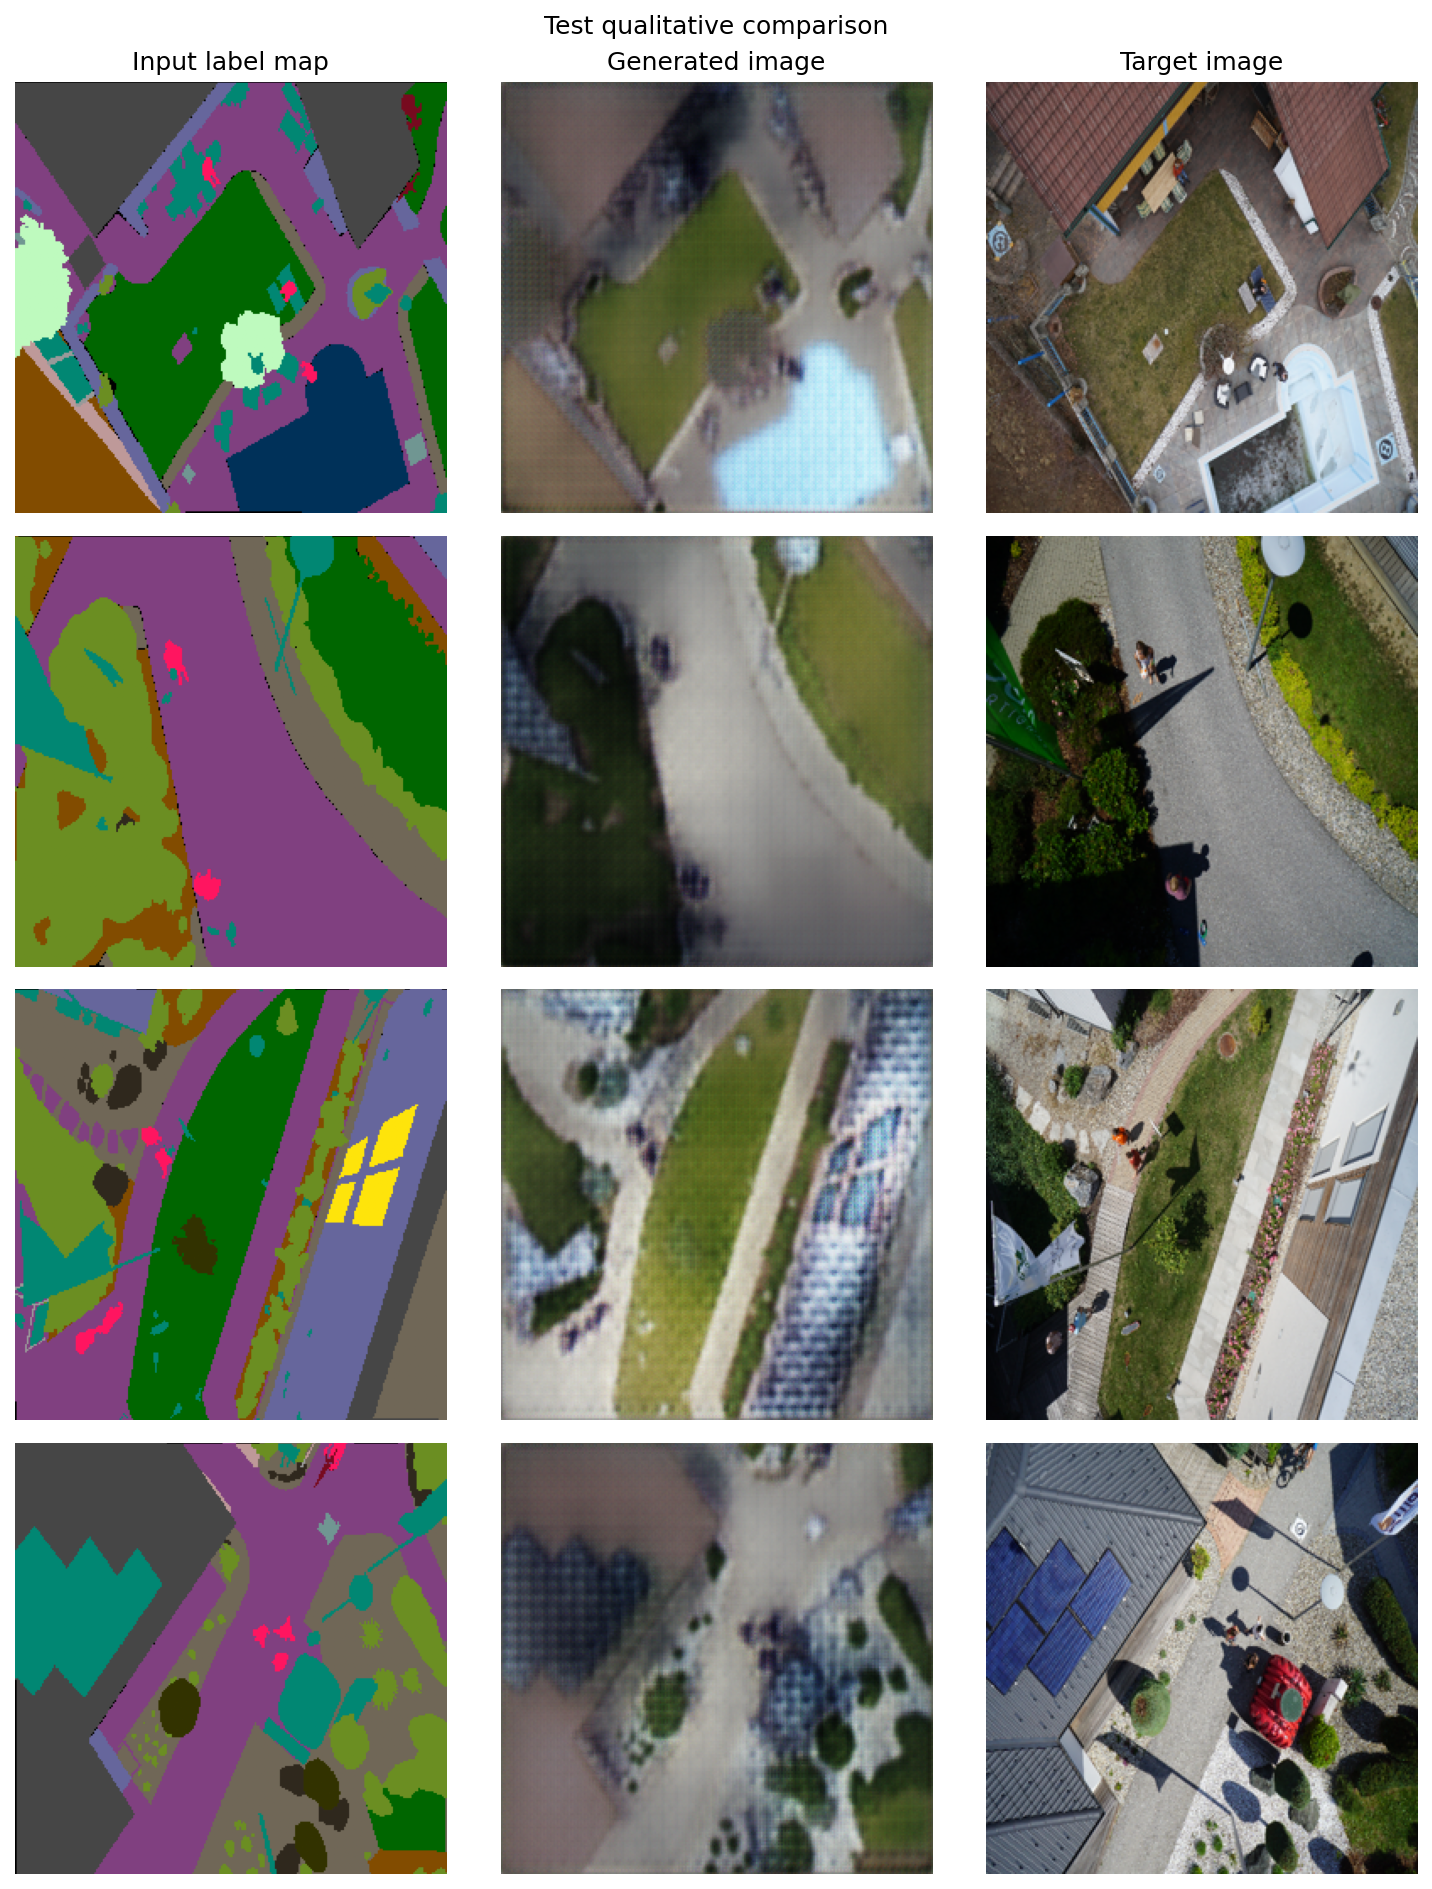
\includegraphics[width=0.98\linewidth]{figures/final_lsgan_l1_100_e40_grid.png}
\caption{LSGAN qualitative grid. Rows show input label map, generated image, and target/reference image.}
\label{fig:lsgan}
\end{figure}

\begin{figure}[H]
\centering
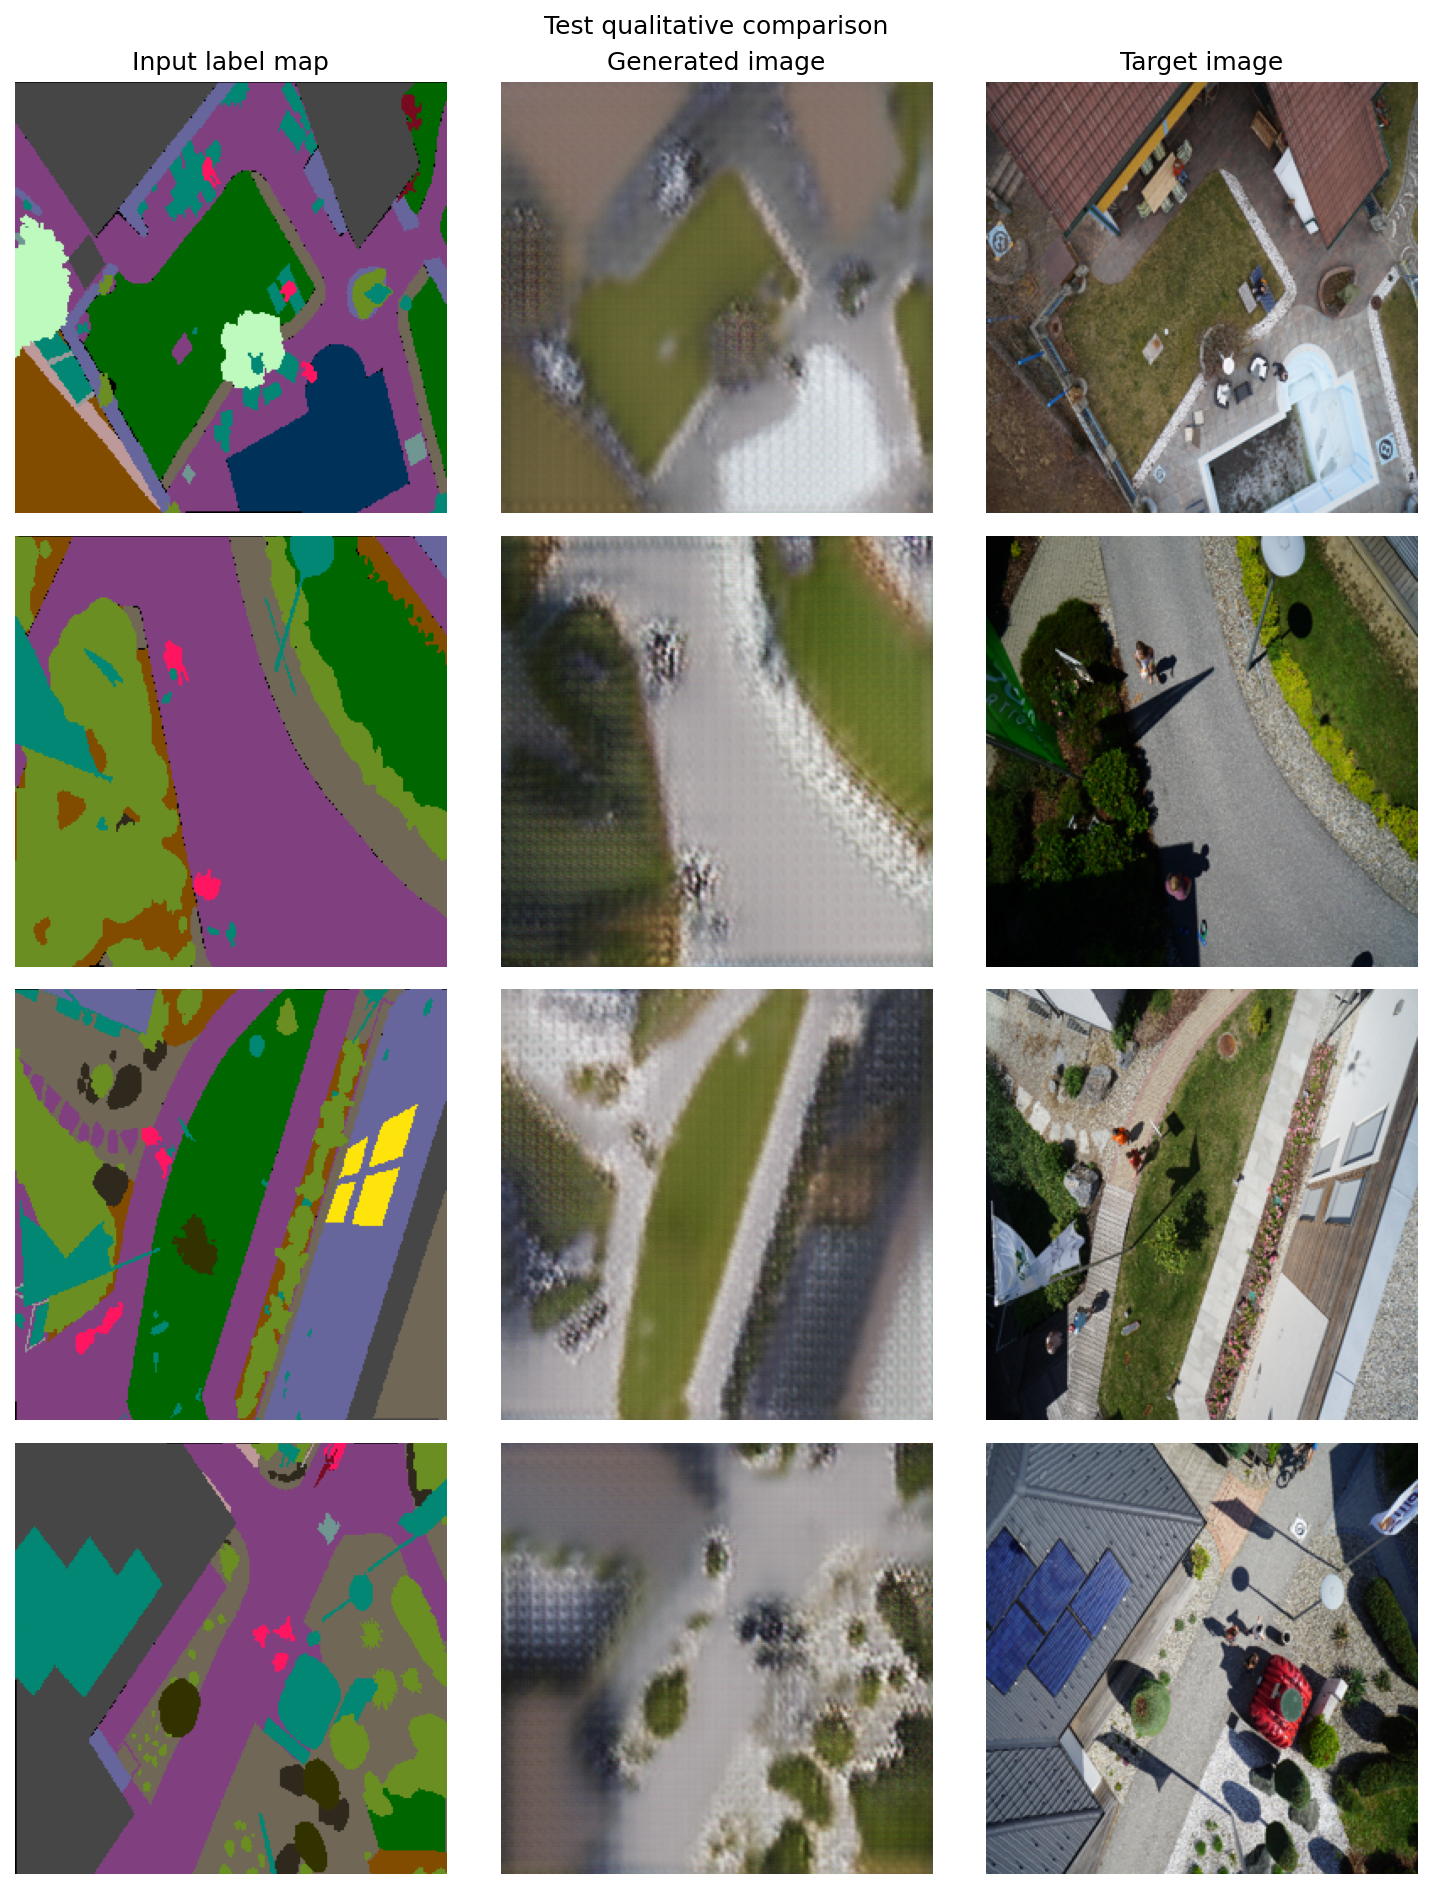
\includegraphics[width=0.98\linewidth]{figures/final_pix2pixhd_lite_ms2_fm10_e40_grid.png}
\caption{Pix2PixHD-lite qualitative grid. The model improves validation MAE but still shows blurry borders and limited high-frequency realism.}
\label{fig:pix2pixhd}
\end{figure}

\begin{figure}[H]
\centering
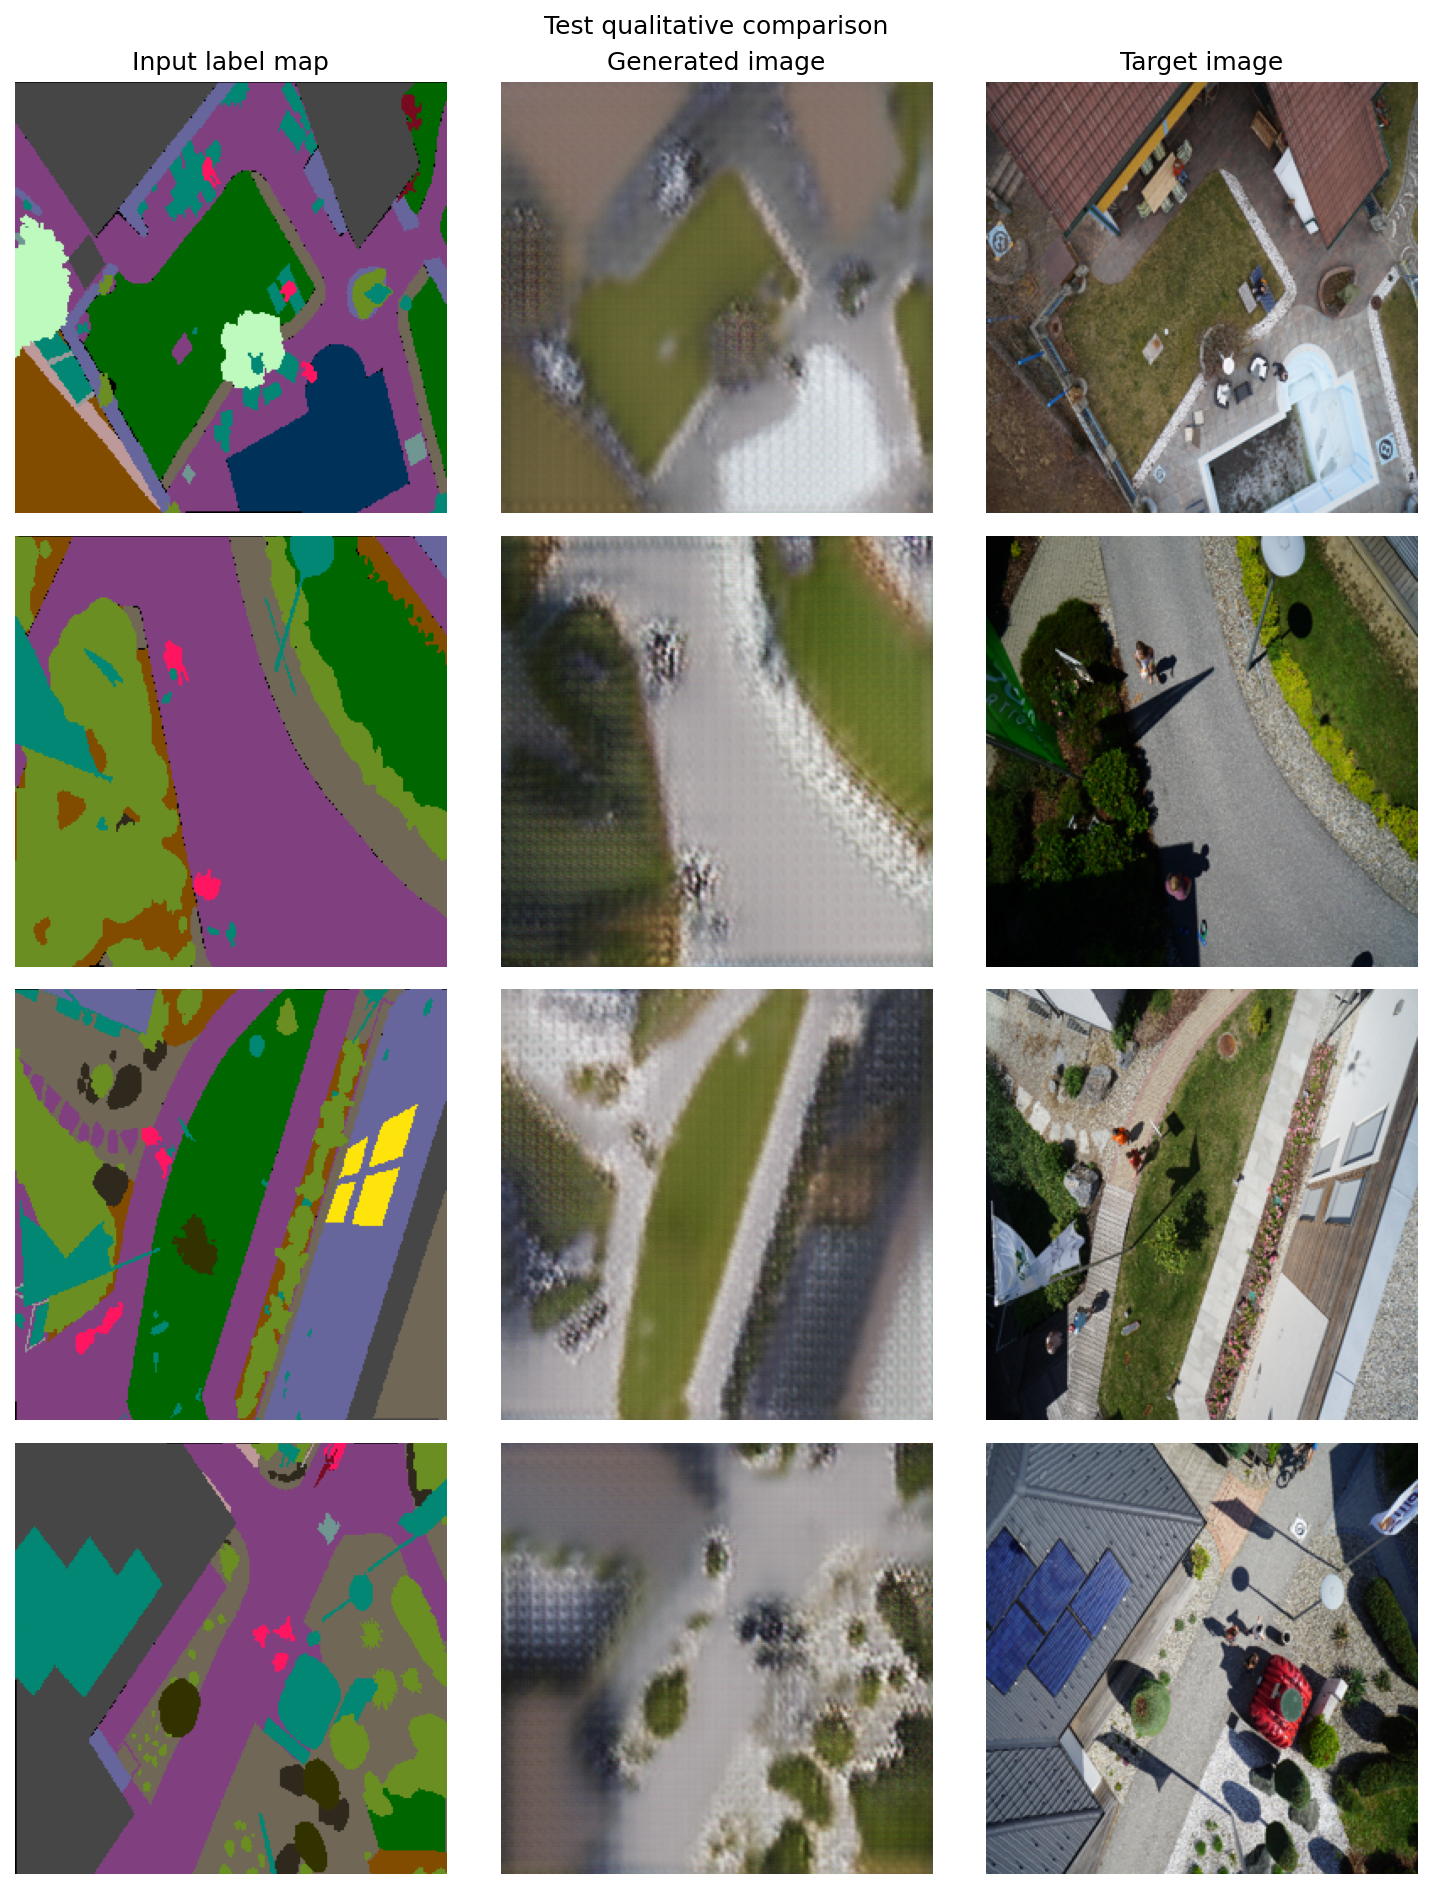
\includegraphics[width=0.98\linewidth]{figures/best_model_current_grid.png}
\caption{Current best-model visual example included for the final discussion. At the time of writing, Pix2PixHD-lite provides the best validation MAE among completed runs. The input label map is respected, but the generated RGB image remains smoother than the real target, especially around semantic borders.}
\label{fig:best-current}
\end{figure}
\FloatBarrier

Qualitatively, the generated images are recognizably conditioned on the label maps, but they are not photorealistic. Borders between semantic regions are often blurred, small people and objects are simplified, and the exact target texture is not recovered. This is partly expected: the input label map contains semantic regions but not the final texture, lighting, or object identity. A larger dataset, stochastic latent conditioning, stronger perceptual losses, or diffusion-style refinement could improve realism.

\section{How to Run}
The commands below are formatted as tables to avoid overflowing the IEEE columns.

\begin{table}[H]
\centering
\resizebox{\columnwidth}{!}{%
\begin{minipage}{\columnwidth}
\caption{Environment and notebook commands.}
\label{tab:run-notebook}
\begin{tabular}{p{0.22\textwidth}p{0.70\textwidth}}
\toprule
Step & Command \\
\midrule
Project root & \code{cd /home/erik/cv2-image-to-image} \\
Activate venv & \code{source .venv/bin/activate} \\
Install dependencies & \code{pip install -r requirements.txt} \\
Run notebook & \code{jupyter notebook notebooks/00\_tutorial\_entrega\_pix2pix.ipynb} \\
\bottomrule
\end{tabular}
\end{minipage}}
\end{table}
\FloatBarrier

\begin{table}[H]
\centering
\resizebox{\columnwidth}{!}{%
\begin{minipage}{\columnwidth}
\caption{Experiment and demo commands.}
\label{tab:run-experiments}
\begin{tabular}{p{0.22\textwidth}p{0.70\textwidth}}
\toprule
Action & Command \\
\midrule
Baseline & \code{python run\_experiment.py baseline} \\
LSGAN & \code{python run\_experiment.py lsgan} \\
Attention & \code{python run\_experiment.py attention} \\
Pix2PixHD-lite & \code{python run\_experiment.py pix2pixhd\_lite} \\
Transfer help & \code{python -m src.train\_transfer --help} \\
Visual demo & \code{python demo/visual\_demo.py --host 0.0.0.0 --port 7860} \\
Browser URL & \code{http://localhost:7860} \\
\bottomrule
\end{tabular}
\end{minipage}}
\end{table}
\FloatBarrier

In the visual demo, use \code{paired-right} for original TU-Graz paired images because the right half is the label map. Use \code{label} when uploading a standalone label map. The optional reference image is only for visual comparison and is not used by the generator.


\section{Conclusion}
This project implements a complete conditional GAN workflow for TU-Graz Landing: clean Python modules, experiment inheritance, reusable metrics, a tutorial notebook, a Gradio demo, and an IEEE-style report. The strongest completed model by validation MAE is Pix2PixHD-lite, while the strongest SSIM among completed runs is obtained by LSGAN. Transfer learning with a ResNet18 encoder almost reaches Pix2PixHD-lite in MAE, which suggests that pretrained visual features help optimization but do not fully solve the semantic-map to aerial-image domain gap.

The main technical conclusion is that this task is generative but highly underdetermined. The input label map specifies class layout, not exact texture, illumination, shadows, or small-object appearance. This explains why outputs can be semantically aligned but still blurry or visibly synthetic. A deterministic U-Net would probably be competitive on MAE, but it would optimize paired reconstruction rather than distributional realism. The adversarial discriminator remains justified because the goal is not only to reproduce one target image, but to synthesize images that look locally plausible.

We intentionally did not prioritize CycleGAN because paired supervision is available. CycleGAN is powerful when domains are unpaired, but here it would ignore the strongest signal in the dataset. The self-attention experiment is the most relevant direction toward transformer-like context modeling under the time and GPU constraints: it preserves convolutional structure while giving the generator a mechanism to connect distant semantic regions. Our expectation is that attention or a future hybrid CNN-transformer generator would be most useful near boundaries, where the current models blur transitions.

Under the time limit, the modified 50-epoch batch is treated as an ablation rather than a definitive leaderboard. The available results indicate that LSGAN with L2 reconstruction improves faster than the reduced-L1 baseline, and attention remains competitive, but these runs require the full schedule before making stronger claims. The best stable delivery result remains Pix2PixHD-lite, supported by both quantitative validation metrics and qualitative inspection.

Future work should include a deterministic U-Net baseline, a larger dataset, stochastic latent conditioning, stronger perceptual losses, and a second-stage refinement model. A transformer-style generator or attention-augmented Pix2PixHD would be a natural next step, especially for improving long-range consistency and semantic boundaries.

\section*{Assisted with Codex}
The project organization, implementation review, experiment orchestration, demo integration, and report drafting were assisted with Codex. All final decisions, interpretation, and submission responsibility remain with the authors.


\begin{thebibliography}{99}

\bibitem{goodfellow2014gan}
I. Goodfellow, J. Pouget-Abadie, M. Mirza, B. Xu, D. Warde-Farley, S. Ozair, A. Courville, and Y. Bengio, ``Generative Adversarial Nets,'' \emph{Advances in Neural Information Processing Systems}, 2014. Available: \url{https://arxiv.org/pdf/1406.2661}

\bibitem{radford2016dcgan}
A. Radford, L. Metz, and S. Chintala, ``Unsupervised Representation Learning with Deep Convolutional Generative Adversarial Networks,'' \emph{International Conference on Learning Representations}, 2016.

\bibitem{mirza2014cgan}
M. Mirza and S. Osindero, ``Conditional Generative Adversarial Nets,'' arXiv:1411.1784, 2014.

\bibitem{isola2017pix2pix}
P. Isola, J.-Y. Zhu, T. Zhou, and A. A. Efros, ``Image-to-Image Translation with Conditional Adversarial Networks,'' \emph{Proceedings of the IEEE Conference on Computer Vision and Pattern Recognition}, 2017.

\bibitem{mao2017lsgan}
X. Mao, Q. Li, H. Xie, R. Y. K. Lau, Z. Wang, and S. P. Smolley, ``Least Squares Generative Adversarial Networks,'' \emph{Proceedings of the IEEE International Conference on Computer Vision}, 2017.

\bibitem{wang2018pix2pixhd}
T.-C. Wang, M.-Y. Liu, J.-Y. Zhu, A. Tao, J. Kautz, and B. Catanzaro, ``High-Resolution Image Synthesis and Semantic Manipulation with Conditional GANs,'' \emph{Proceedings of the IEEE Conference on Computer Vision and Pattern Recognition}, 2018.

\bibitem{zhang2019sagan}
H. Zhang, I. Goodfellow, D. Metaxas, and A. Odena, ``Self-Attention Generative Adversarial Networks,'' \emph{International Conference on Machine Learning}, 2019.

\bibitem{ronneberger2015unet}
O. Ronneberger, P. Fischer, and T. Brox, ``U-Net: Convolutional Networks for Biomedical Image Segmentation,'' \emph{Medical Image Computing and Computer-Assisted Intervention}, 2015.

\bibitem{he2016resnet}
K. He, X. Zhang, S. Ren, and J. Sun, ``Deep Residual Learning for Image Recognition,'' \emph{Proceedings of the IEEE Conference on Computer Vision and Pattern Recognition}, 2016.

\bibitem{ganvariants}
G. Iglesias, E. Talavera, and A. Diaz-Alvarez, ``A survey on GANs for computer vision: Recent research, analysis and taxonomy,'' \emph{Computer Science Review}, vol. 48, 100553, 2023. Available: \url{https://arxiv.org/pdf/2203.11242}

\bibitem{wang2004ssim}
Z. Wang, A. C. Bovik, H. R. Sheikh, and E. P. Simoncelli, ``Image Quality Assessment: From Error Visibility to Structural Similarity,'' \emph{IEEE Transactions on Image Processing}, vol. 13, no. 4, pp. 600--612, 2004.

\bibitem{wang2003msssim}
Z. Wang, E. P. Simoncelli, and A. C. Bovik, ``Multiscale Structural Similarity for Image Quality Assessment,'' \emph{The Thirty-Seventh Asilomar Conference on Signals, Systems and Computers}, 2003.

\bibitem{lopezpaz2017c2st}
D. Lopez-Paz and M. Oquab, ``Revisiting Classifier Two-Sample Tests,'' \emph{International Conference on Learning Representations}, 2017.

\bibitem{sajjadi2018precision}
M. S. M. Sajjadi, O. Bachem, M. Lucic, O. Bousquet, and S. Gelly, ``Assessing Generative Models via Precision and Recall,'' \emph{Advances in Neural Information Processing Systems}, 2018.

\bibitem{kynkaanniemi2019improved}
T. Kynkaanniemi, T. Karras, S. Laine, J. Lehtinen, and T. Aila, ``Improved Precision and Recall Metric for Assessing Generative Models,'' \emph{Advances in Neural Information Processing Systems}, 2019.

\bibitem{heusel2017fid}
M. Heusel, H. Ramsauer, T. Unterthiner, B. Nessler, and S. Hochreiter, ``GANs Trained by a Two Time-Scale Update Rule Converge to a Local Nash Equilibrium,'' \emph{Advances in Neural Information Processing Systems}, 2017.

\bibitem{karras2019stylegan}
T. Karras, S. Laine, and T. Aila, ``A Style-Based Generator Architecture for Generative Adversarial Networks,'' \emph{Proceedings of the IEEE/CVF Conference on Computer Vision and Pattern Recognition}, 2019.

\end{thebibliography}

\end{document}
